\section{Diseño del Videojuego}\label{sec:diseño}

Antes de explicar en detalle el diseño del videojuego debemos tener en cuenta que el objetivo principal es diseñar e implementar un juego en el que la toma de decisiones juegue un papel fundamental. La finalidad de esta investigación es analizar si un videojuego puede influir a los jugadores en las decisiones que toman o no, para ello se le planteará un dilema moral inicial al jugador, y dependiendo de su respuesta, el juego y su historia trataran de influenciar al jugador para hacerlo cambiar de opinión.

Las mecánicas a describir se plantean como un conjunto de minijuegos que apoyan a la historia en los diferentes espacios a los que el jugador puede llegar dependiendo de las decisiones que tome. Con esta información en mente, procederemos a explicar el diseño del videojuego y cada uno de los elementos que lo componen.

Para facilitar la compresión del documento, se presentará primero la narrativa del videojuego antes de continuar con el resto de los elementos que la apoyan y complementan.


%\textbf{CREO QUE DEBES HACER UNA BREVE INTRODUCCIÓN PARA PONER EN CONTEXTO AL LECTOR. PRESENTAS DIRECTAMENTE Y SIN ESA INTRODUCCIÓN RESULTA DIFICIL SABER DE DONDE SALEN LAS COSAS. TE HAGO UNA PROPUESTA Y TU MISMO REPASALA}

%Antes de entrar en detalle en la descripción del diseño del videojuego debemos tener en cuenta que nuestro objetivo es diseñar e implementar un videojuego en el que la toma de decisiones juegue un papel fundamental. Como tema de dilema el juego se centrará en el suicidio. Por tanto nos interesará que las decisiones que tome el jugador en torno a este tema queden integradas en la historia del juego. La idea es plantear un dilema moral inicial al jugador, en nuestro caso \textit{se suicida el protagonista o no}, y dependiendo de su respuesta, el videojuego y su historia trataran de influenciar al jugador para cambiar su opción. 

%La mecánica principal del juego se plantea como un conjunto de mini-juegos que se asociaran a diferentes espacios a los que se llegará en función de las decisiones que tome el jugador.  Sobre estos espacios se definirá una narrativa con unos personajes asociados que nos dará sentido a los diferentes recorridos que podrá seguir el jugador.  Con esta información en mente, a continuación explicaremos el diseño del videojuego y cada uno de los elementos que lo componen. Para facilitar la comprensión de las diferentes mecánicas de juego presentaremos en primer lugar la narrativa asociada al juego y a continuación entraremos en detalle en las mecánicas. 

%\textbf{mini-juegos siempre con guión}

%%%%%%%%%%%%%%%%%%%%%%%%%%%%%%%%%%%%%%%%%%%%%%%%%%%%

\subsection{Narrativa}

En esta sección se dará el contexto bajo el cuál está enmarcado el juego. Se presentaran los personajes y los distintos escenarios en los que actuarán junto con un resumen adecuado de la historia.

\subsubsection{Contexto y personajes}
La historia se sitúa en el tiempo contemporáneo, año 2019/2020 en una ciudad que se encuentra al interior del país. La familia de la protagonista es de clase media-alta. Ganan lo suficiente para poder pagar las cosas que necesita su hija, pero viven más alejados del centro de la ciudad, lo que hace que los tiempos de viaje entre el hogar y la universidad sean de 1 hora - 1 hora y 30 minutos en transporte público.

Los personajes que aparecen a lo largo de la historia son los siguientes:

\subsubsection{Protagonista: Lucía}
Lucía es la protagonista de la historia. En el juego sigues su historia y ves como los distintos sucesos la van afectando.

\begin{itemize}
    \item \textbf{Edad:} 20 años
    \item \textbf{Género:} Femenino
    \item \textbf{Contextura Física:} Joven de estatura media (1.64m) y contextura muy delgada. Su es cabello liso y de color castaño claro. Suele ir con vestimenta formal debido a las exigencias de su carrera y su familia.
    \item \textbf{Características Psicológicas:} Solitaria y sin amigos. Disfruta de la música y las artes aunque hoy en día no tiene tiempo para ello. No suele sonreír mucho y se la pasa estresada y con ansiedad producto de la presión de sus padres y la universidad.
\end{itemize}

\begin{figure}[h]
    \centering
    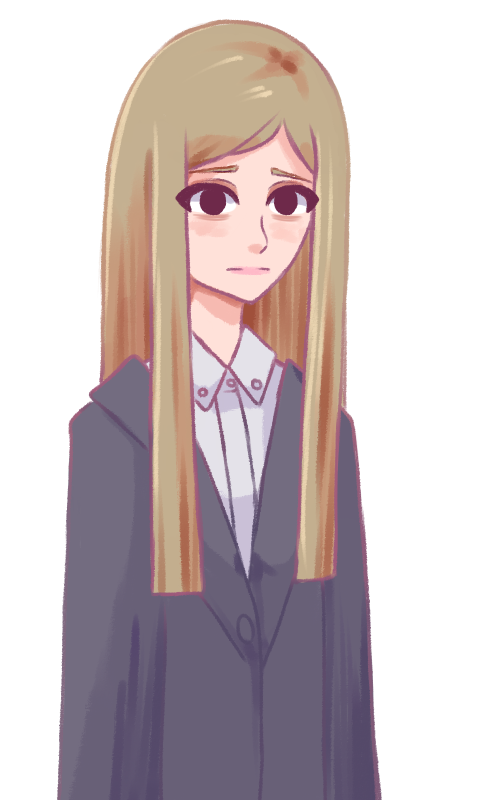
\includegraphics{imgs/lucia.png}
    \caption{Retrato de Lucía}
    \label{fig:lucia}
\end{figure}

\subsubsection{Secundario: La Muerte}
Personaje secundario. Actúa como mensajero para Lucía en la ruta donde la chica está muerta. Le ayuda a desvelar los misterios y las memorias detrás de su muerte.

\begin{itemize}
    \item \textbf{Edad:} Desde el inicio de los tiempos.
    \item \textbf{Género:} -
    \item \textbf{Contextura Física:} Además de una capucha con un moño, no se ve nada más de su persona.
    \item \textbf{Características Psicológicas:} Ente totalmente neutro que ayuda a las almas a encontrar su paz. Provee de nuevos puntos de vista a Lucía.
\end{itemize}

\begin{figure}[h]
    \centering
    
\includegraphics{imgs/muerte.png}
    \caption{Retrato de La Muerte}
    \label{fig:muerte}
\end{figure}

\newpage
\subsubsection{Secundario: Profesor de la Universidad}
Personaje secundario. Muestra el paso de Lucía por la universidad y el estrés al cuál se ve enfrentada ella.

\begin{itemize}
    \item \textbf{Edad:} 47 años
    \item \textbf{Género:} Masculino
    \item \textbf{Contextura Física:} Hombre de estatura algo más alta que el promedio (1.76m) y de contextura media. Pelo corto y de color oscuro. Suele ir siempre ordenado con camisa y corbata.
    \item \textbf{Características Psicológicas:} Abogado que ejerce de profesor en la universidad sin tener ningún tipo de educación pedagógica. En su clase él es quien tiene la verdad y tiene la última palabra.
\end{itemize}

\begin{figure}[h]
    \centering
    
\includegraphics{imgs/profe.png}
    \caption{Retrato del Profesor}
    \label{fig:profesor}
\end{figure}




\subsubsection{Escenarios}
\paragraph{Hogar de Lucía}
El lugar donde reside nuestra protagonista junto a sus dos padres. La casa es de ladrillos y está compuesta por dos pisos, en el piso de abajo se encuentran la cocina, sala de estar y comedor, mientras que en el piso de arriba se encuentran los dormitorios de la protagonista, y de sus padres.

Los eventos que transcurren en este lugar se centran principalmente en la habitación de Lucía, donde se le ve un poco en su intimidad pero que funciona principalmente como lugar de estudio (y estrés producto de la carga académica de su carrera). Adicionalmente es el lugar donde Lucía recupera sus memorias.

\begin{figure}[ht]
	\centering
	\begin{minipage}{0.45\textwidth}
   		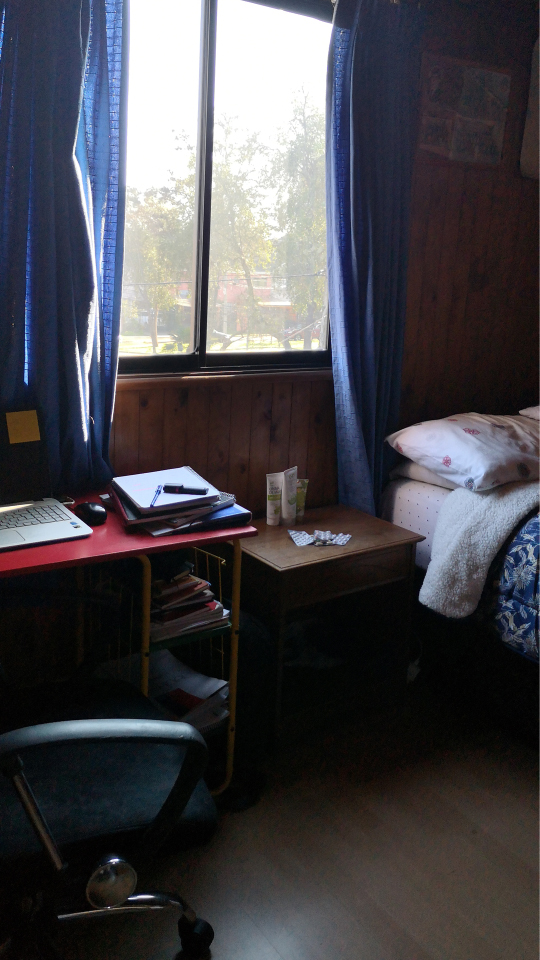
\includegraphics[scale=.3]{imgs/habitacion.jpg}
	\end{minipage}
	\begin{minipage}{0.45\textwidth}
		\begin{flushright}
	   		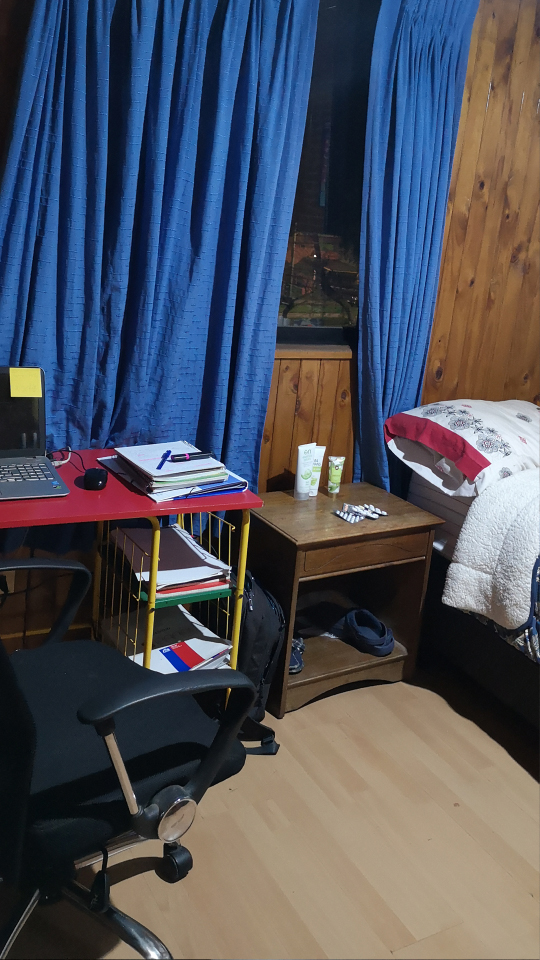
\includegraphics[scale=.3]{imgs/habitacion-noche.jpg}
		\end{flushright}
	\end{minipage}
	\caption{Habitación de Lucía in-game}
	\label{multifig:habitacion}
\end{figure}

\paragraph{Universidad}
Los sucesos ocurren concretamente en la facultad de derecho de una universidad de prestigio dentro del país.

Es un lugar que genera estrés y ansiedad a nuestra protagonista, a causa de la alta exigencia que la carrera y la facultad pone en sus estudiantes. Lucía no tiene amigos aquí por lo que los eventos se centran en sus clases, y concretamente en los exámenes que tiene.

\begin{figure}[ht]
    \centering
    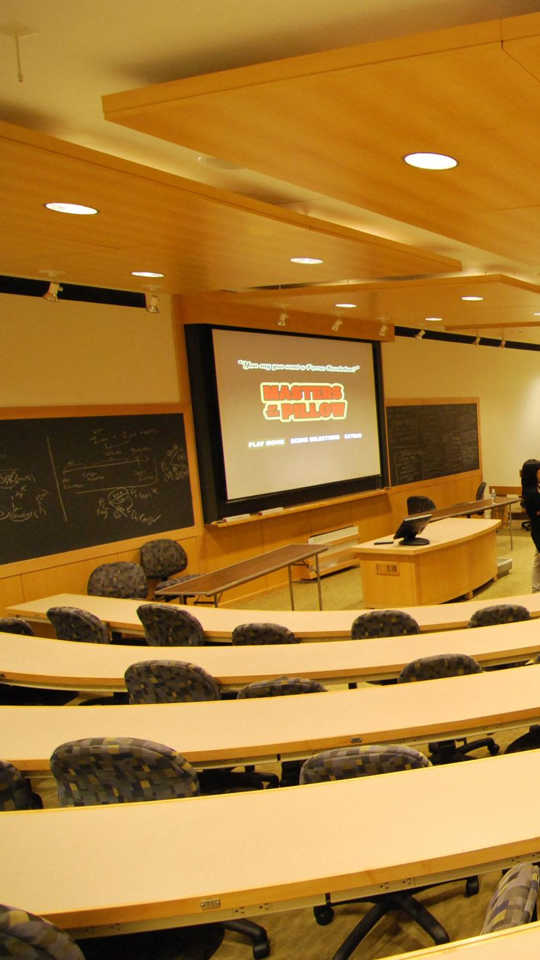
\includegraphics[scale=.3]{imgs/sala-de-clases.jpg}
    \caption{Sala de Clases in-game}
    \label{fig:sala-de-clases}
\end{figure}

\newpage
\paragraph{Vías del Tren}
Lugar que trae paz y calma a nuestra protagonista. Las vías del tren son un lugar donde Lucía solía jugar de joven, y que hoy en día recurre a él cada vez que se siente estresada, con ansiedad, o cuando quiere huir, gracias a que sus padres no tienen conocimiento de este lugar.

Las vías están lo suficientemente aisladas de los caminos para ser un lugar apenas visitado por las personas, los trenes pasan puntualmente cada hora, los árboles, rocas, y algo de pasto son los elementos que normalmente acompañan este paisaje.

Es el sitio donde ocurre la muerte de Lucía.

\begin{figure}[ht]
    \centering
    \begin{minipage}{.24\textwidth}
        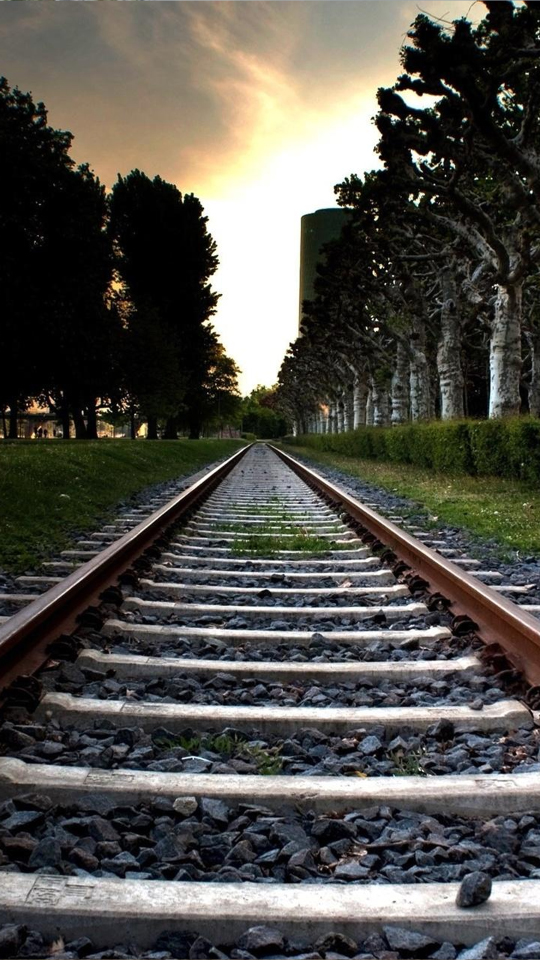
\includegraphics[width=.9\textwidth]{imgs/vias.jpg}
    \end{minipage}
    \begin{minipage}{.24\textwidth}
        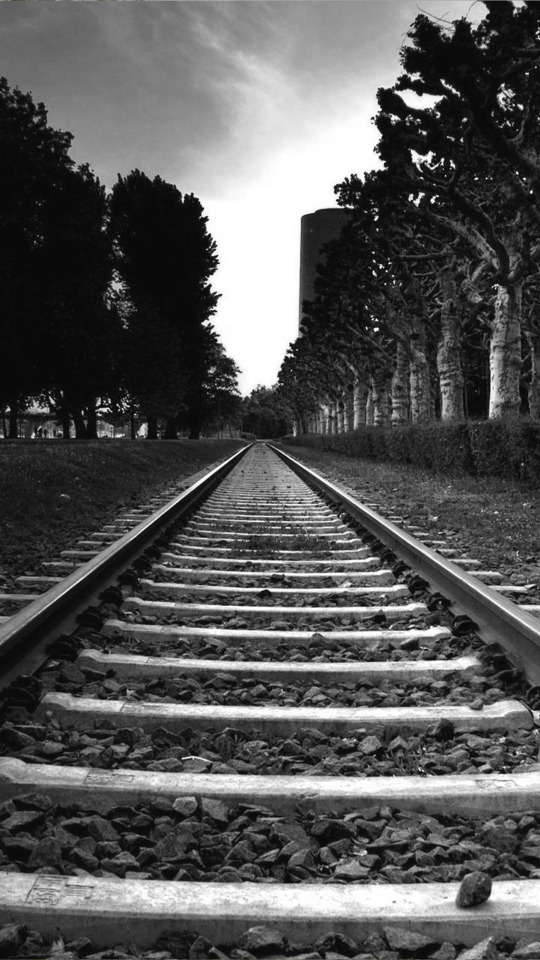
\includegraphics[width=.9\textwidth]{imgs/vias-gris.jpg}
    \end{minipage}
    \begin{minipage}{.24\textwidth}
        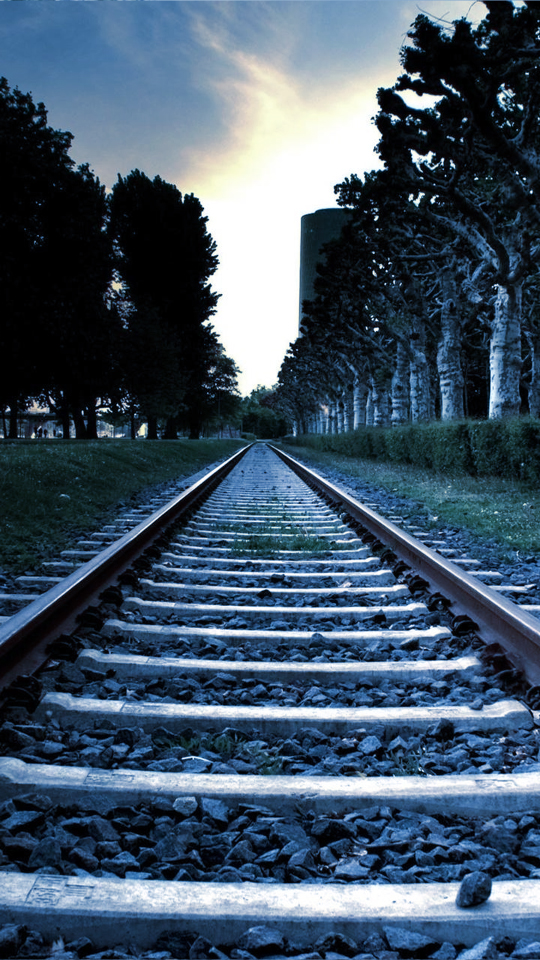
\includegraphics[width=.9\textwidth]{imgs/vias-pasado.jpg}
    \end{minipage}
    \begin{minipage}{.24\textwidth}
        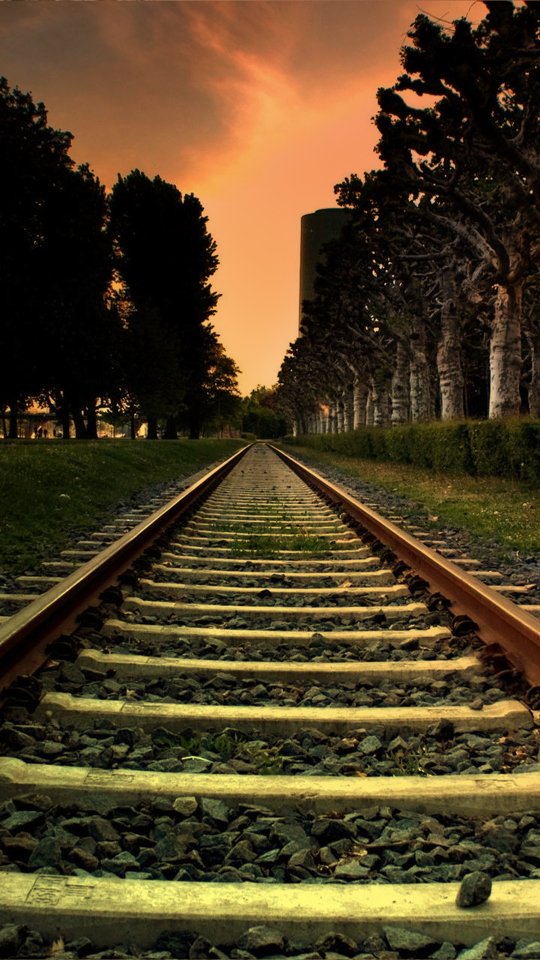
\includegraphics[width=.9\textwidth]{imgs/vias-tarde.jpg}
    \end{minipage}
    \caption{Vías del Tren in-game}
    \label{multifig:vias}
\end{figure}

\subsubsection{Resumen}
Pantalla en negro, texto blanco. Palabras y oraciones nos aparecen en frente sin formar mucho sentido hasta que llegas a una pregunta. \emph{¿La dejas morir?}

A partir de esta pregunta nacen dos lineas narrativas principales: La chica está viva y la acompañas en su día a día, o la chica ha muerto y debes descubrir por qué. En la Figura~\ref{fig:espacios} se muestran un esquema de estas dos lineas y la relación entre ellas. 

\begin{figure}[h]
    \centering
    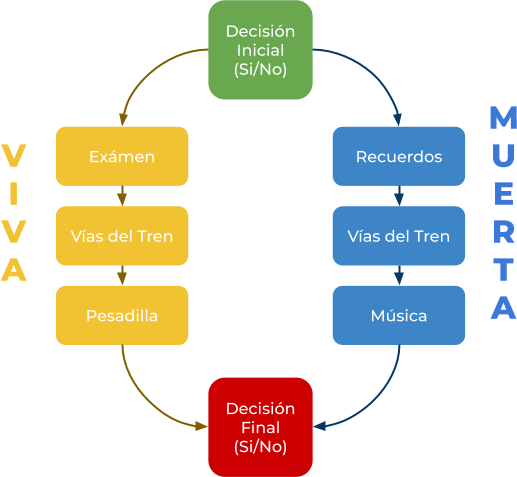
\includegraphics[scale=.6]{imgs/espacios.png}
    \caption{Esquema de Espacios}
    \label{fig:espacios}
\end{figure}

\vspace{.5cm}

\paragraph{La chica vive}
Sigues la historia de Lucía, una chica de clase media-alta que se ha levantado temprano para poder estudiar, son las 4 am y tiene examen a las 8.30. Tiene una pequeña conversación consigo misma, estudia durante un par de horas y luego parte hacia su examen.

Llega a la universidad, se sienta alejada de los demás y comienza a rendir su examen. Lee las preguntas una y otra vez, el reloj avanza pero Lucía no, los alumnos comienzan a irse uno por uno hasta que quedan solo Lucía y el profesor en la sala. El estrés la termina sobrepasando y huye de la sala sin decir nada.

Lucía opta por saltarse el resto de sus clases y emprende rumbo a las vías del tren, el único lugar acogedor para ella en todo el mundo. Pasa un par de horas ahí, ve como pasan los trenes mientras se habla a sí misma, no le gusta su carrera ni disfruta lo que hace pero tampoco tiene más opciones.

Regresa a casa más temprano de lo usual, toma una ducha para terminar de calmar su mente e intenta estudiar nuevamente ya que al día siguiente tiene otro examen más, no obstante, la cabeza no la ayuda para nada así que opta por irse a dormir.

Despierta desvelada e irritada a la mañana siguiente, sufrió de pesadillas durante toda la noche y el examen era la menor de sus preocupaciones, por lo que toma sus cosas y va hacía las vías del tren en lugar de ir a la universidad.

Estando ahí la chica grita y libera todas las emociones que tenía contenidas, la rabia, la pena, el enojo, el rechazo. El reloj avanza, el tren se acerca y Lucía grita cada vez más y más fuerte hasta que debes tomar una decisión.

Si decides que Lucía muera, esta saltará a las vías justo cuando el tren este por pasar, tan puntual como siempre, tan exacto como ella conoce. Después de esto el juego muestra como una pequeña flor creció en el punto donde Lucía decidió terminar con su vida.

Si decides que Lucía siga viva, en lugar de saltar a las vías del tren decide huir. No le ve ningún sentido a continuar con la misma vida que ha tenido hasta ahora, por lo que emprende un nuevo viaje sin decirle nada a nadie, desapareciendo sin dejar rastro.

\paragraph{La chica muere}
La pantalla está en tonos azulados, se ve la línea del tren de fondo y puedes notar como el tiempo está congelado, la protagonista se encuentra confundida, no sabe qué ha ocurrido. Pasan los minutos, un portal aparece y de este, emerge ``La Muerte''.

La Muerte le explica a Lucía que se ha ido del mundo terrenal antes de que fuese su tiempo, por tanto su alma no ha quedado en paz y no puede encontrar el camino por sí sola.

Al ver a Lucía aún confundida, La Muerte le invita a averiguar el porqué de su muerte y le extiende una mano mientras abre un nuevo portal. 

El primer lugar que visitan es la habitación de Lucía, en ella se encuentran distintas piezas brillando en el piso de la habitación. La Muerte le indica a Lucía que esos son trozos de distintos recuerdos de ella, y que se acerque a verlos más de cerca. 

Lucía está confundida, esperaba solo recuerdos malos pero hubieron algunos que le traían felicidad. La Muerte le explica que como el ser imparcial que es debe mostrarle todos los matices de su vida, no solo lo malo, es por eso que los recuerdos estaban mezclados para que Lucía pueda entender mejor todas las aristas de su vida.

Se abre otro portal, y La Muerte lleva a Lucía a ver una versión de sí misma, pero más joven. Están en las vías del tren, se ve como la pequeña se divierte corriendo, saltando, y jugando con las rocas, las hojas, y con todo lo que aquella zona le ofrecía para hacerlo.

Lucía suspira, le causa ternura verse a sí misma sin ningún tipo de problema ni preocupación. La Muerte le explica que las cosas no eran tan distintas, si bien Lucía tenía problemas, siempre tuvo un lugar donde desahogarse, un lugar que le permitía encontrar paz y alivio, y que le ofrecía ser feliz. Ven a la pequeña un par de momentos más y luego se van por otro portal.

Llegan nuevamente a la habitación de Lucía, solo que esta vez no estaban solos, una Lucía algo más joven que se encontraba practicando con su guitarra les hacía compañía. 
 
A Lucía le causa nostalgia aquella imagen, comenta como esa fue la última vez que disfruto de la música como tal, sin embargo, La Muerte le corrige: ``No fue la última, puesto que ahora también has disfrutado con ella''. Se quedan hasta que la canción de la Lucía más joven termina, y después ambas almas se van a través de otro portal.
 
Finalmente regresan al punto de inicio donde La Muerte encontró a Lucía, y le ofrece un trato. No suele hacerlo pero le ofrece a Lucía una segunda oportunidad para vivir, puede volver al momento anterior a su muerte con todo el conocimiento que ha aprendido hasta ahora, o puede irse con ella y pasar al siguiente plano.

Si decides que Lucía vuelva a la vida, se verá como ella está de pie al lado de las vías justo cuando el tren está pasando. Lucía toma la decisión de que si bien ha vuelto a la vida, no quiere volver a pasar por lo mismo que antes, por lo que huye de la ciudad y desaparece sin dejar rastro.

Si decides que Lucía se mantenga muerta, ves como La Muerte abre un último portal, por donde se van tanto ella como Lucía, sin decir nada más.

%%%%%%%%%%%%%%%%%%%%%%%%%%%%%%%%%%%%%%%%%%%%%%%%%%%%

\subsection{Mecánicas}
Las mecánicas se han definido a partir de los diferentes espacios de la historia presentada. Cada una de estos espacios se ha transformado en un espacio de juego.

\subsubsection{Espacios de Juego}
Los espacios de juego hacen referencia a los distintos escenarios en los cuales se situará al jugador. Para efectos de este proyecto estos espacios hacen referencia principalmente a los minijuegos que se le presentarán al jugador a lo largo de la historia. La descripción de los minijuegos sigue el esquema presentado en la Figura~\ref{fig:espacios}.  Para cada uno de los espacios presentaremos la interacción del jugador y la mecánica asociada.

\paragraph{Decisión Inicial}
La pantalla está en negro, aparece una breve historia y una pregunta al final del todo.
\begin{center} \textbf{¿Salvas a la chica?} \end{center}

Es la primera interacción del juego e influye en cómo se desarrolla el resto del mismo.

\begin{figure}[ht]
	\centering
	\begin{minipage}{0.45\textwidth}
   		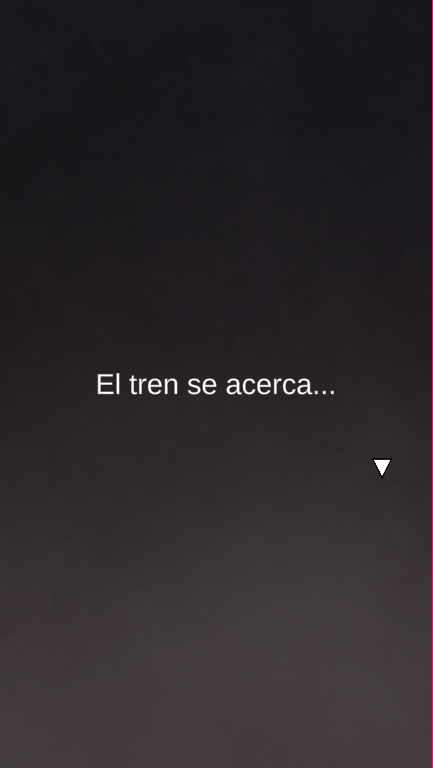
\includegraphics[scale=.5]{imgs/screenshot01.png}
	\end{minipage}
	\begin{minipage}{0.45\textwidth}
		\begin{flushright}
	   		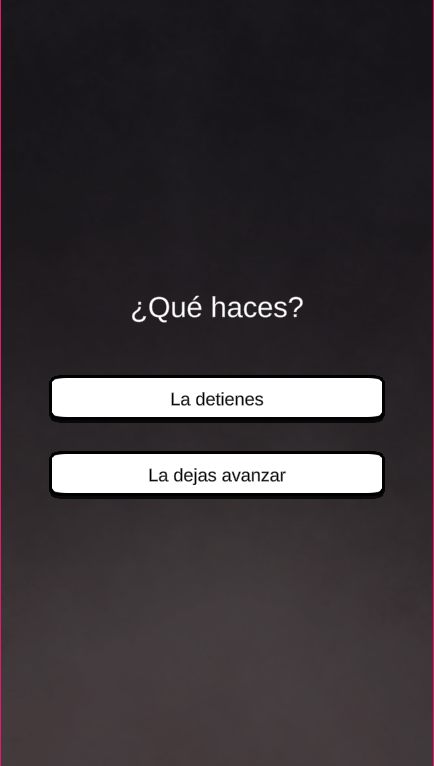
\includegraphics[scale=.5]{imgs/screenshot02.png}
		\end{flushright}
	\end{minipage}
	\caption{Screenshots de la decisión}
	\label{multifig:decision}
\end{figure}

\paragraph{Decisión Final}
Este espacio es similar al anterior, la pregunta se repite una vez más y marca el final del juego. La mayor diferencia es que el jugador tiene mucha más información de la historia y los personajes, pero la pregunta en esencia es la misma.

\paragraph{Viva: Examen}
Estás dando el examen y debes mantener tu cabeza libre de pensamientos intrusivos. Tienes una barra de feedback en la parte superior de la pantalla que te indica que tan estresada estás, y debes mantener la barra lo más bajo posible.

\textbf{Debes:} Tocar y arrastrar los pensamientos fuera de tu cabeza.

Los pensamientos que aparecen son adjetivos o frases que desmotivan a Lucía o la desvalorizan como persona.
\begin{center}
    \textit{Estrés, Ansiedad, Angustia, Ignorante, Incapaz, Miedo, Soy Nadie, No Valgo}
\end{center}

\begin{figure}[h]
	\centering
	\begin{minipage}{0.45\textwidth}
   		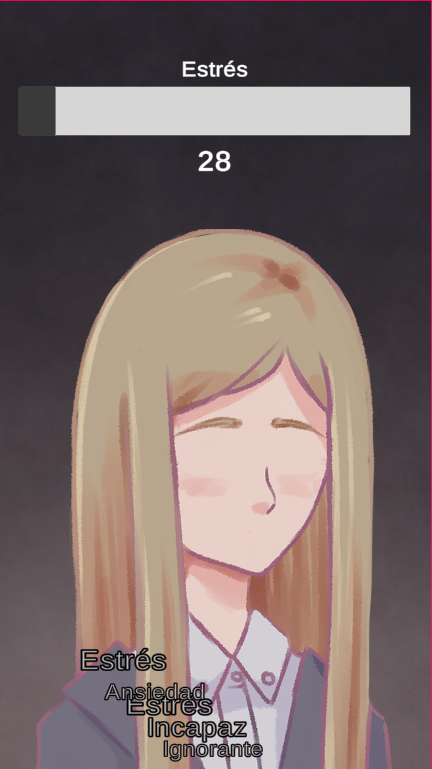
\includegraphics[scale=.5]{imgs/screenshot03.png}
	\end{minipage}
	\begin{minipage}{0.45\textwidth}
		\begin{flushright}
	   		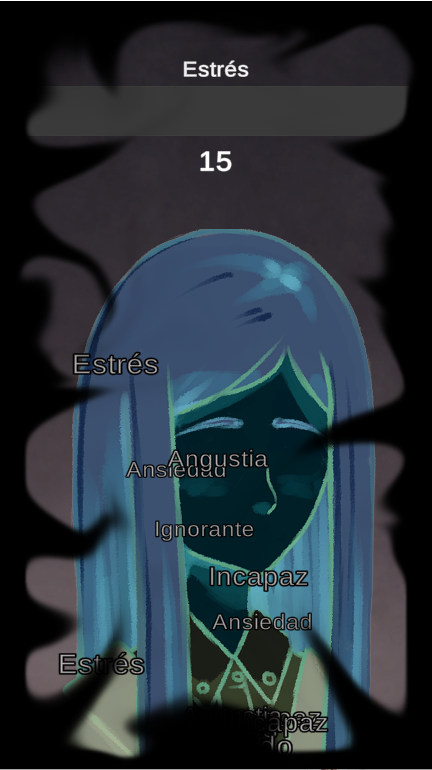
\includegraphics[scale=.5]{imgs/screenshot04.png}
		\end{flushright}
	\end{minipage}
	\caption{Screenshots del examen}
	\label{multifig:examen}
\end{figure}

\newpage
\paragraph{Viva: Vías del Tren}
En este escenario, Lucía trata de calmarse después de todo el estrés que le han causado las situaciones anteriores. Tienes una barra de feedback en la parte superior de la pantalla que te indica lo estresada que estás, debes mantenerla lo más bajo posible para que Lucía recobre la calma.

\textbf{Debes:} Tocar y arrastrar las hojas a las tablas y mantener la misma cantidad de hojas en cada una de las tablas del tren.

%Tu meta es juntar la misma cantidad de hojas en cada una de las tablas del tren.
\begin{figure}[h]
    \centering
    \begin{minipage}{0.45\textwidth}
        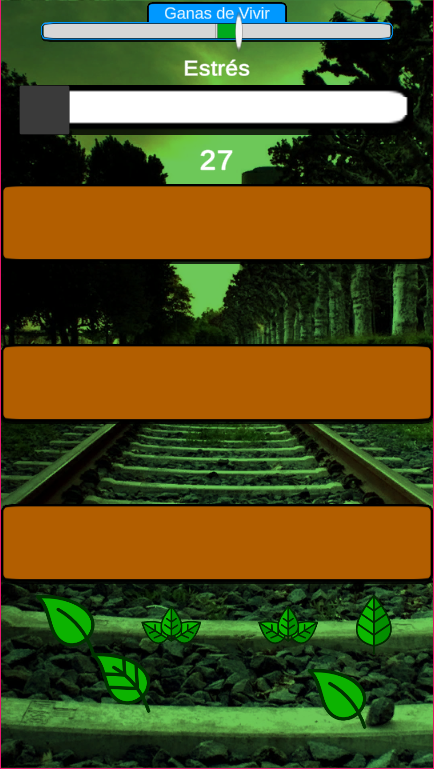
\includegraphics[scale=.5]{imgs/screenshot11.png}
    \end{minipage}
    \begin{minipage}{0.45\textwidth}
        \begin{flushright}
            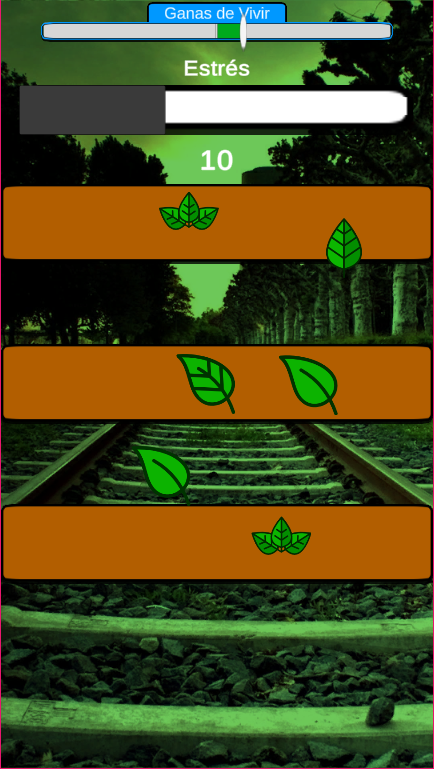
\includegraphics[scale=.5]{imgs/screenshot12.png}
        \end{flushright}
    \end{minipage}
    \caption{Screenshots de las vías}
    \label{multifig:calma}
\end{figure}

\newpage
\paragraph{Viva: Pesadilla}
En este escenario Lucía tiene una pesadilla y debe sobrevivir a ella. La pantalla se torna oscura y con distintos destellos que dan la sensación de que la oscuridad te va comiendo. La jugabilidad es la de un pequeño \textit{runner} donde debes esquivar los obstáculos del camino hasta llegar a la meta.

\textbf{Debes:} Tocar la pantalla para saltar los obstáculos.

La meta se representa como una pequeña barra en la parte superior de la pantalla que va avanzando a medida que Lucía huye de la pesadilla.


\begin{figure}[h]
	\centering
	\begin{minipage}{0.45\textwidth}
   		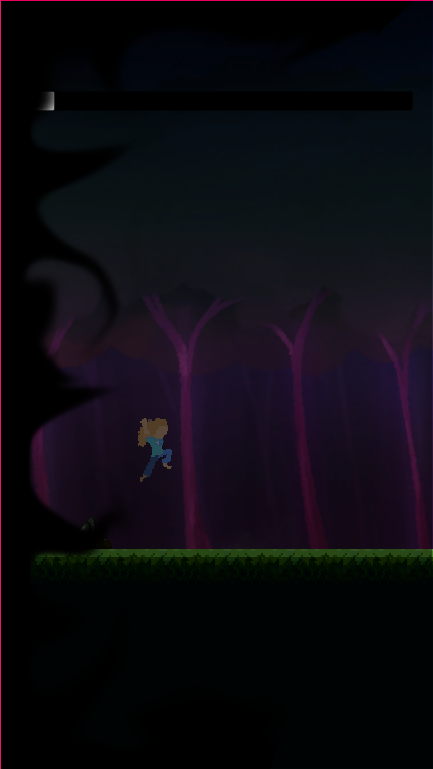
\includegraphics[scale=.5]{imgs/screenshot05.png}
	\end{minipage}
	\begin{minipage}{0.45\textwidth}
		\begin{flushright}
	   		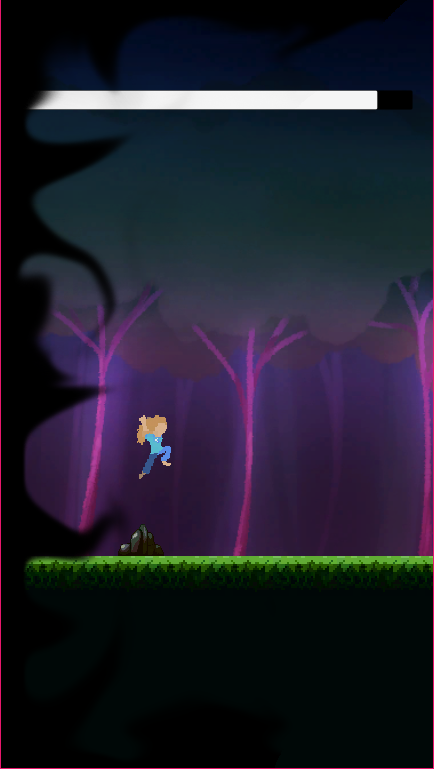
\includegraphics[scale=.5]{imgs/screenshot06.png}
		\end{flushright}
	\end{minipage}
	\caption{Screenshots de la pesadilla}
	\label{multifig:pesadilla}
\end{figure}

\newpage
\paragraph{Muerta: Recuerdos}
En este escenario Lucía se encuentra muerta y con la ayuda de la muerte trata de recordar porqué está muerta. El minijuego se trata de resolver los puzzles para armar la imagen y recuperar sus recuerdos.

El jugador puede presionar un botón en la parte superior de la pantalla para ver la imagen completa como pista y así guiarse al armar el puzzle.

\textbf{Debes:} Tocar y arrastrar las piezas para armar la imagen.

Los recuerdos que recupera son: \textit{Soledad, Estrés y Pasión por la Música}\\
Estos recuerdos son seleccionados para mostrar lo malo de la vida de Lucía, pero también para ver que no todo era tan malo.

\begin{figure}[h]
	\centering
	\begin{minipage}{0.45\textwidth}
   		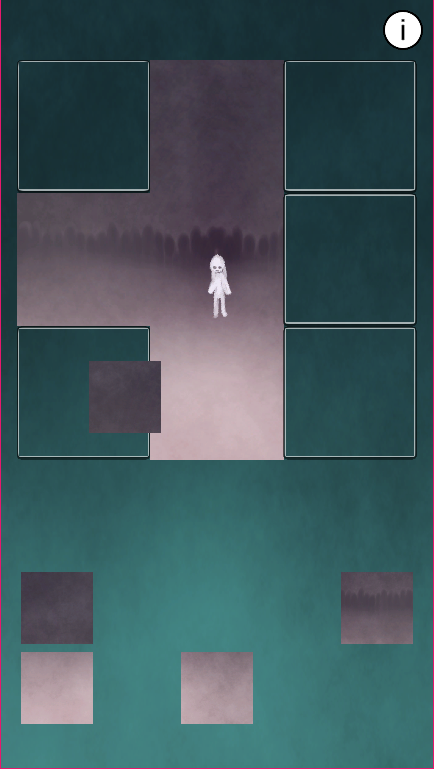
\includegraphics[scale=.5]{imgs/screenshot07.png}
	\end{minipage}
	\begin{minipage}{0.45\textwidth}
		\begin{flushright}
	   		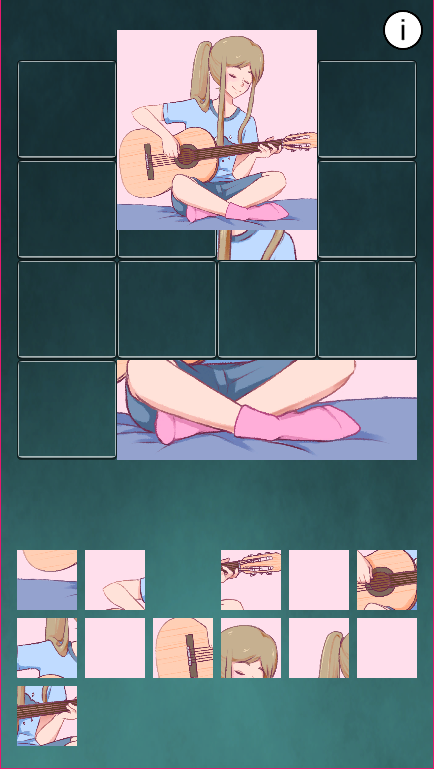
\includegraphics[scale=.5]{imgs/screenshot08.png}
		\end{flushright}
	\end{minipage}
	\caption{Screenshots de los puzzles}
	\label{multifig:recuerdos}
\end{figure}

\newpage
\paragraph{Muerta: Lucía Pequeña}
En este escenario Lucía regresa en el tiempo para ver una versión más pequeña de sí misma. En este minijuego se ve a la pequeña Lucía feliz y sonriente mientras juega al correr.

El jugador controla a la Lucía pequeña y debe recolectar la mayor cantidad de flores que pueda antes de llegar a la meta, la cuál está representada como una barra en la parte superior de la pantalla que va avanzando.

\textbf{Debes:} Tocar la pantalla para que Lucía salte y recolecte las flores.

\begin{figure}[h]
	\centering
	\begin{minipage}{0.45\textwidth}
   		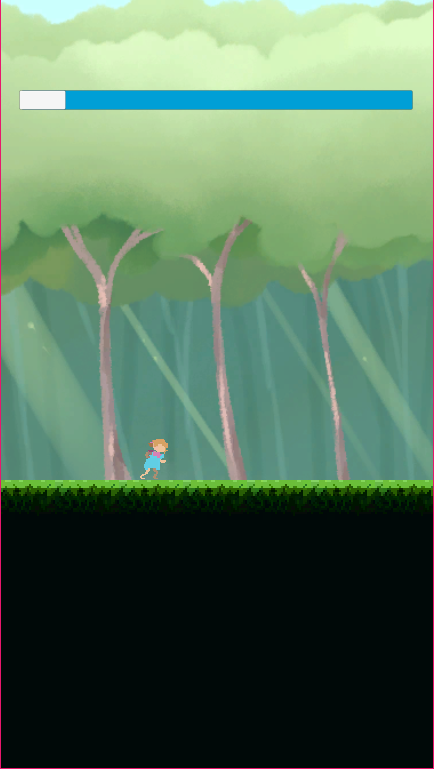
\includegraphics[scale=.5]{imgs/screenshot09.png}
	\end{minipage}
	\begin{minipage}{0.45\textwidth}
		\begin{flushright}
	   		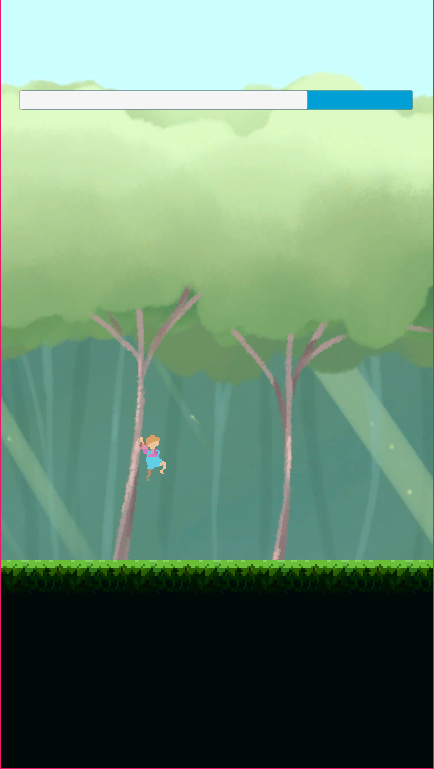
\includegraphics[scale=.5]{imgs/screenshot10.png}
		\end{flushright}
	\end{minipage}
	\caption{Screenshots de Lucía Pequeña}
	\label{multifig:pequeña}
\end{figure}

\newpage
\paragraph{Muerta: Música}
En este escenario Lucía y la Muerte vuelven a la habitación de la chica, donde encuentran una Lucía viva disfrutando de la música.
Este minijuego emula al ``Simón Dice'', donde en la pantalla se muestra una secuencia y el jugador la debe imitar.

\textbf{Debes:} Tocar los botones en el orden indicado.

\begin{figure}[h]
	\centering
	\begin{minipage}{0.45\textwidth}
   		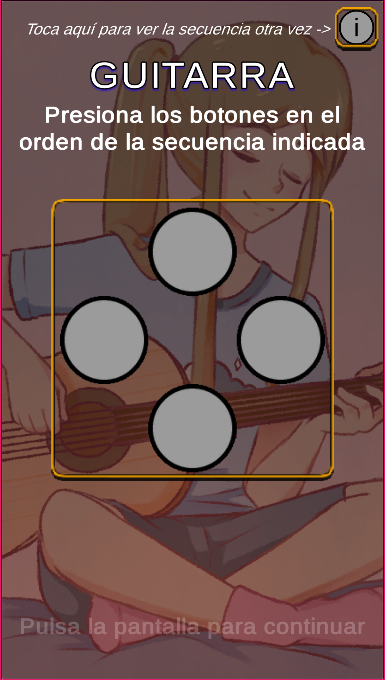
\includegraphics[scale=.5]{imgs/screenshot13.png}
	\end{minipage}
	\begin{minipage}{0.45\textwidth}
		\begin{flushright}
	   		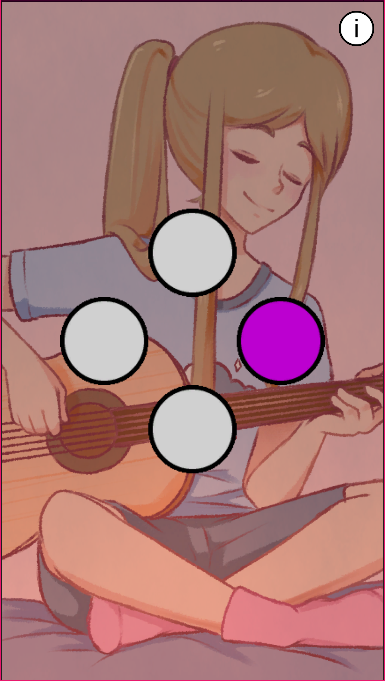
\includegraphics[scale=.5]{imgs/screenshot14.png}
		\end{flushright}
	\end{minipage}
	\caption{Screenshots de Lucía Musical}
	\label{multifig:musica}
\end{figure}

\newpage
\subsubsection{Economía del Juego}\label{sec:economia}
El juego se centra en las emociones de la protagonista, y la economía del mismo se basa en torno a eso.

La ``moneda'' central que se utiliza son las \textbf{Ganas de Vivir}. Estas aumentan o disminuyen según cada minijuego en particular, dependiendo de si Lucía está viva, o está muerta.

\begin{table}[ht]
    \centering
    \begin{tabular}{|x|p{13cm}|}
        \hline
        \textbf{\Gls{sources}} & La chica vive\\
        & \textbf{Vías del tren:} Genera tranquilidad, aumenta ganas de vivir\\
        \cline{2-2}
        & La chica muere\\
        & \textbf{Recuerdos:} Genera alivio, aumenta las ganas de vivir.\\
        & \textbf{Música:} Genera relajo, aumenta las ganas de vivir.\\
        & \textbf{Lucía Pequeña:} Genera nostalgia, aumenta las ganas de vivir.\\
        \hline
        \textbf{\Gls{drains}} & La chica vive\\
        & \textbf{Examen:} Genera estrés, disminuye las ganas de vivir.\\
        & \textbf{Pesadilla:} Genera miedo, disminuye las ganas de vivir.\\
        \cline{2-2}
        & La chica muere\\
        & \textbf{Recuerdos:} Genera angustia, disminuye las ganas de vivir.\\
        \hline
        \textbf{\Gls{converters}} & La generación de las distintas emociones \textit{(Tranquilidad, alivio, relajo, nostalgia, estrés, miedo, angustia)} afectan directamente a las ganas de vivir de Lucía.\\
        \hline
        \textbf{\Gls{traders}} & \\
        \hline
    \end{tabular}
    \caption{Economía del Juego}
    \label{tab:economia}
\end{table}


%%%%%%%%%%%%%%%%%%%%%%%%%%%%%%%%%%%%%%%%%%%%%%%%%%%%

\subsection{Interfaces}\label{sec:interfaces}

A continuación se explicará la paleta de colores y los fondos utilizados en el videojuego. Posteriormente veremos cada una de las pantallas del mismo y los elementos gráficos que componen su interfaz visual.

\subsubsection{Paleta de Colores}
Para mostrar el deterioro del estado mental de Lucía y los oscuro que se ve su mundo, se enfocó principalmente en utilizar una paleta de colores oscura y con poca saturación.

\begin{figure}[ht]
    \centering
    \begin{minipage}{.45\textwidth}
        \centering
        
\includegraphics[width=.9\textwidth]{imgs/fondox.png}
        \caption{Fondo Genérico}
        \label{fig:fondo-generico}
    \end{minipage}
    \begin{minipage}{.5\textwidth}
        \begin{minipage}{.45\textwidth}
            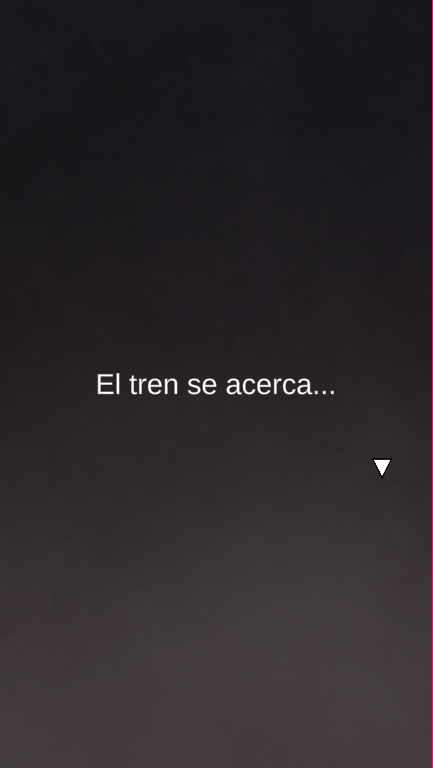
\includegraphics[width=\textwidth]{imgs/screenshot01.png}
        \end{minipage}
        \begin{minipage}{.45\textwidth}
            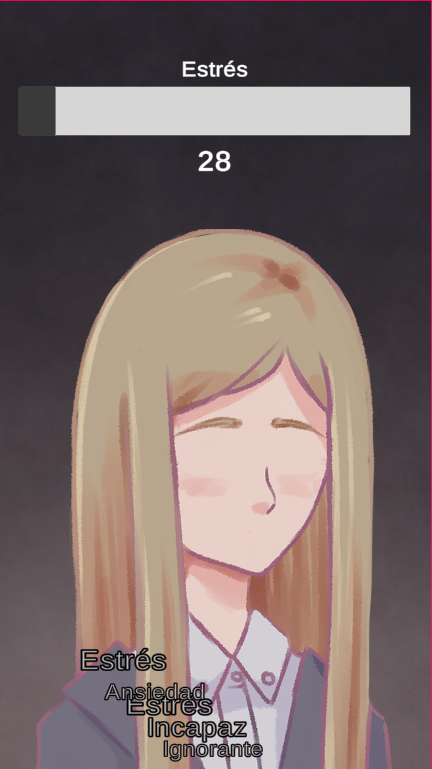
\includegraphics[width=\textwidth]{imgs/screenshot03.png}
        \end{minipage}
        \caption{Fondo Usado in-game}
        \label{fig:fondo-generico-in-game}
    \end{minipage}
\end{figure}

Además de los tonos oscuros, los fondos son ambiguos y los colores se mezclan entre si, dando una sensación de confusión e incerteza (Figuras~\ref{fig:mal-recuerdo} y~\ref{fig:fondo-pesadilla}).
\begin{figure}[ht]
    \centering
    \begin{minipage}{.34\textwidth}
        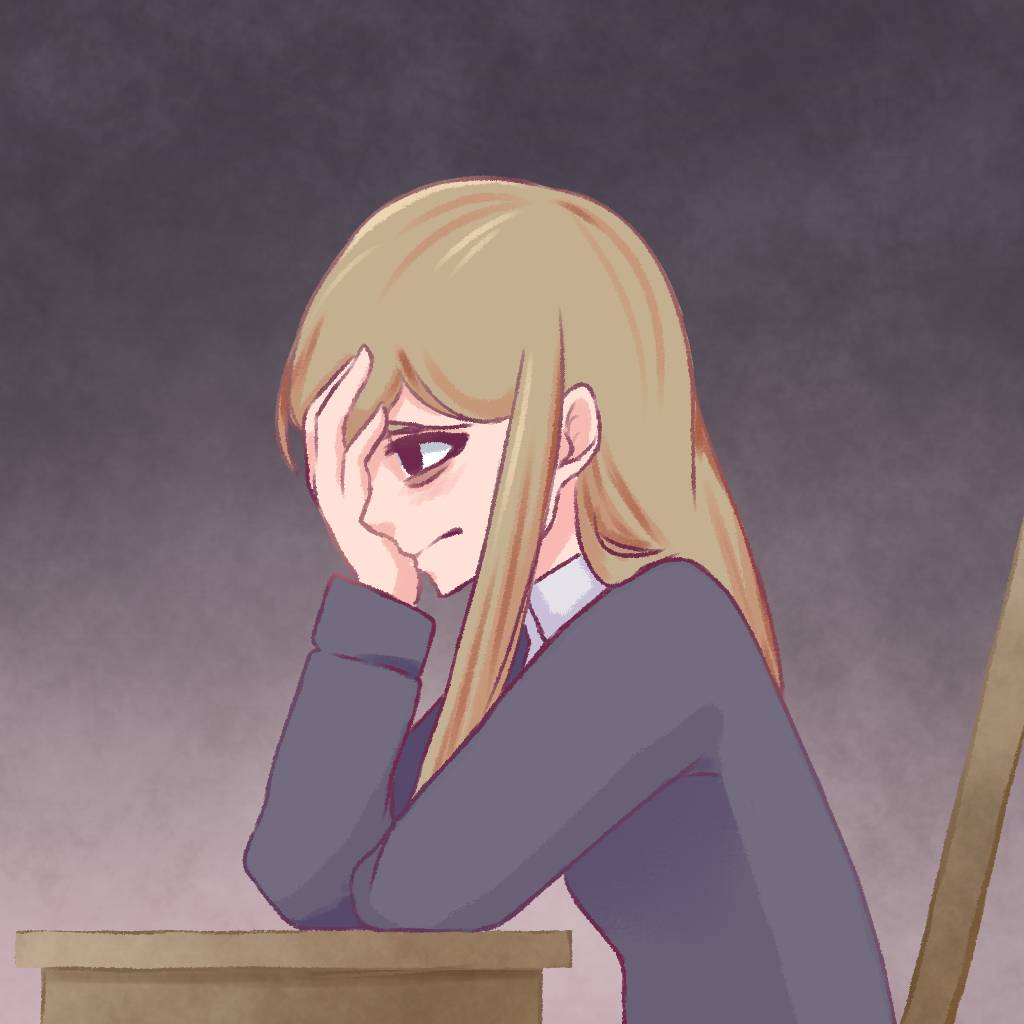
\includegraphics[width=.95\textwidth]{imgs/Memory1.png}
        \caption{Mal Recuerdo}
        \label{fig:mal-recuerdo}
    \end{minipage}
    \begin{minipage}{.65\textwidth}
        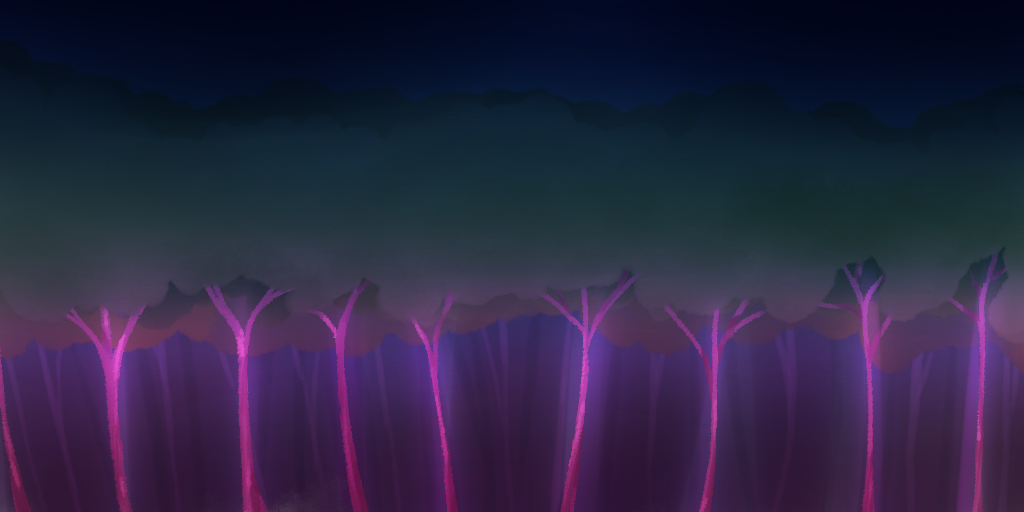
\includegraphics[width=\textwidth]{imgs/bg_pesadilla.png}
        \caption{Fondo Pesadilla}
        \label{fig:fondo-pesadilla}
    \end{minipage}
\end{figure}

Por otro lado, cuando se ven las cosas buenas en la vida de Lucía o sus buenos recuerdos, se busca dar una sensación de comodidad. Los fondos se tornan más definidos así como también la paleta de colores se vuelve más luminosa utilizando tonos pastel (Figuras~\ref{fig:buen-recuerdo} y~\ref{fig:fondo-pequeña}).
\begin{figure}[ht]
    \centering
    \begin{minipage}{.34\textwidth}
        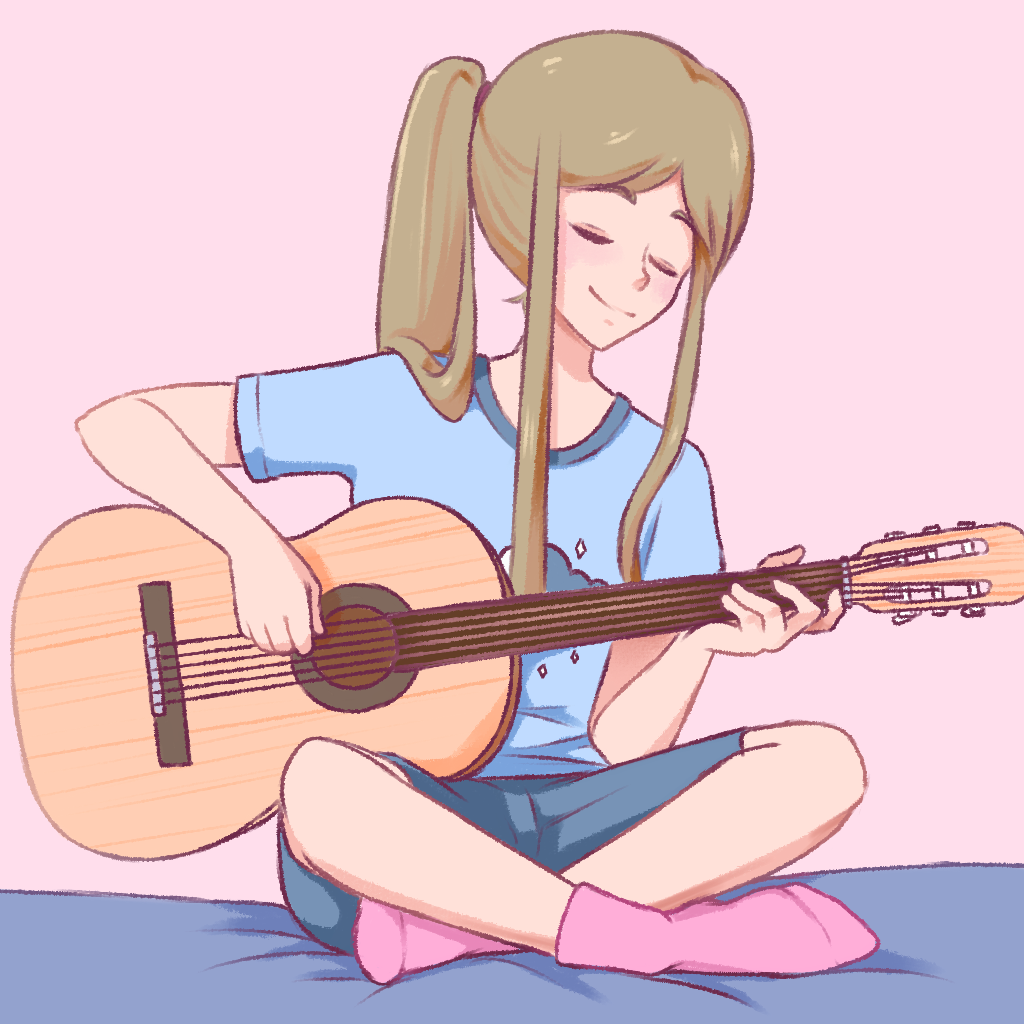
\includegraphics[width=.95\textwidth]{imgs/Memory3.png}
        \caption{Buen Recuerdo}
        \label{fig:buen-recuerdo}
    \end{minipage}
    \begin{minipage}{.65\textwidth}
        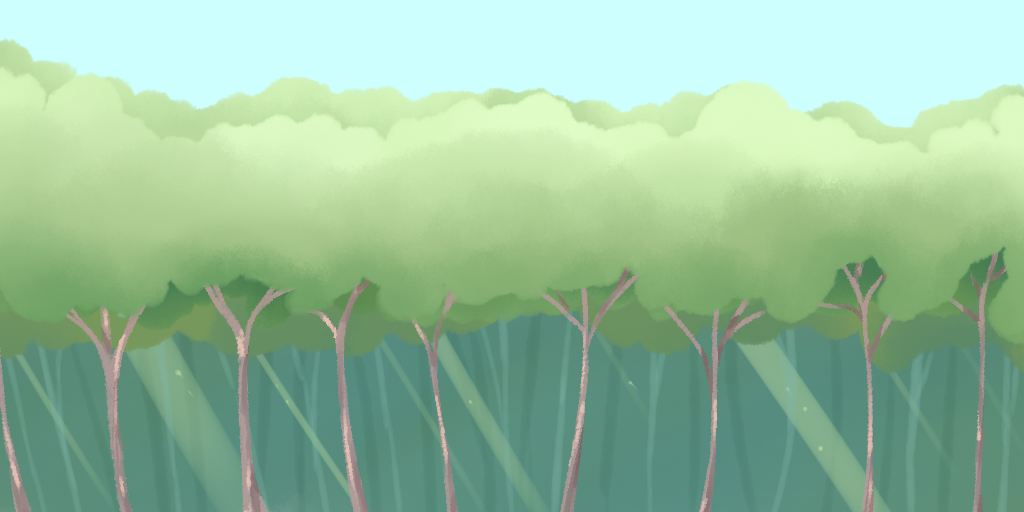
\includegraphics[width=\textwidth]{imgs/bg.png}
        \caption{Fondo Lucía Pequeña}
        \label{fig:fondo-pequeña}
    \end{minipage}
\end{figure}

Para acompañar esto en todo momento, se utiliza una interfaz plana con colores blancos y negros para los textos y los diálogos. Esto permite que el resto de los elementos en pantalla (fondos y retratos del personaje) decidan la emoción y la sensación a transmitir al jugador.

%\begin{figure}[h]
%    \begin{minipage}{.45\textwidth}
%        \centering
%        
\includegraphics[scale=.5]{imgs/textbox.png}
%    \end{minipage}
%    \begin{minipage}{.45\textwidth}
%        \centering
%        
\includegraphics[scale=.5]{imgs/nameplate.png}
%    \end{minipage}
%    \caption{Interfaces de Diálogo}
%    \label{fig:interfaz-dialogos}
%\end{figure}

\newpage
\subsubsection{Pantallas}\label{sec:pantallas}
\begin{figure}[ht]
    \centering
    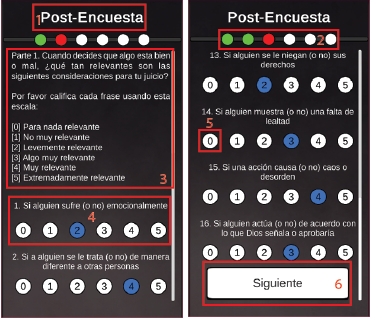
\includegraphics{imgs/hud-encuesta.png}
    \caption{Interfaz: Encuesta}
    \label{fig:hud-encuesta}
\end{figure}

Iniciamos con la pantalla que se muestra al realizarle la encuesta al jugador (Figura~\ref{fig:hud-encuesta}). En esta se pueden encontrar los siguientes elementos:\\
1.- \textbf{Titulo:} El Titulo de la encuesta (Pre o Post Encuesta).\\
2.- \textbf{Barra de Progresión:} Nos indica cuantas pantallas llevamos y cuantas nos faltan para terminar la encuesta.\\
3.- \textbf{Instrucciones:} La instrucciones de como debe responder el jugador.\\
4.- \textbf{Pregunta:} La pregunta de la encuesta.\\
5.- \textbf{Elección:} Botón para realizar la elección del jugador de 0 a 5.\\
6.- \textbf{Siguiente:} Botón para avanzar a la siguiente pantalla.

\newpage
\begin{figure}[ht]
    \centering
    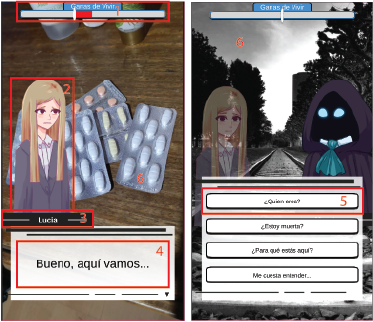
\includegraphics{imgs/hud-narrativa.png}
    \caption{Interfaz: Narrativa}
    \label{fig:hud-narrativa}
\end{figure}

En la Figura~\ref{fig:hud-narrativa} se aprecia la pantalla de narrativa, en la cual se pueden encontrar los siguientes elementos:\\
1.- \textbf{Ganas de vivir:} Es la ``moneda'' del juego, representa las ganas de vivir que tiene Lucía en esos momentos, es afectada por el desempeño en los minijuegos y por las decisiones que tomas (Para más información, revisar la sección \ref{sec:economia}).\\
2.- \textbf{Retrato:} Imagen gráfica del personaje que está hablando actualmente.\\
3.- \textbf{Letrero:} Nombre del personaje que está hablando actualmente.\\
4.- \textbf{Cuadro de Texto:} Espacio donde aparecen los diálogos del juego.\\
5.- \textbf{Botón:} Botón interactuable, aparecen cuando debes tomar una decisión.\\
6.- \textbf{Fondo:} Otorga información contextual del lugar físico en el que se desenvuelve la escena.

\newpage
\begin{figure}[ht]
    \centering
    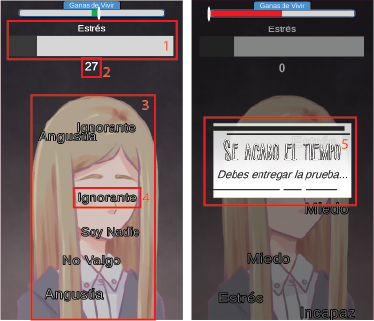
\includegraphics{imgs/hud-examen.png}
    \caption{Interfaz: Examen}
    \label{fig:hud-examen}
\end{figure}

La Figura~\ref{fig:hud-examen} nos muestra las pantallas del minijuego del examen, en el cuál podemos encontrar los siguientes elementos:\\
1.- \textbf{Barra de Estrés:} Muestra lo estresada que está Lucía, es un indicador de lo bien o mal que lo estamos haciendo en el minijuego.\\
2.- \textbf{Tiempo:} Muestra el tiempo restante antes de que el minijuego termine.\\
3.- \textbf{Zona de Juego:} Esta es la zona donde aparecen nuevas palabras.\\
4.- \textbf{Palabra:} Palabra que rebota dentro de la zona de juego y representa un pensamiento intrusivo para Lucía.\\
5.- \textbf{Cuadro de Game Over:} Cuadro que indica que el minijuego ha acabado, y que puedes continuar con la historia.

\newpage
\begin{figure}[ht]
    \centering
    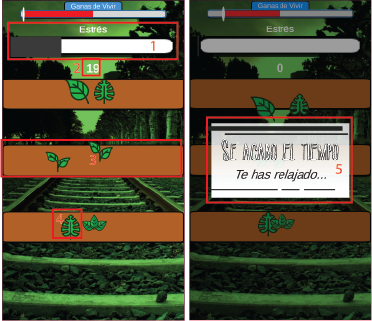
\includegraphics{imgs/hud-vias.png}
    \caption{Interfaz: Vías}
    \label{fig:hud-vias}
\end{figure}

La Figura~\ref{fig:hud-vias} muestra las pantallas del minijuego de las vías del tren. Los elementos aquí son:\\
1.- \textbf{Barra de Estrés:} Muestra lo relajada que está Lucía, es un indicador de lo bien o malo que lo estamos haciendo en el minijuego.\\
2.- \textbf{Tiempo:} Muestra el tiempo restante antes de que el minijuego termine.\\
3.- \textbf{Vía:} Zona a la cuál el jugador debe mover las hojas.\\
4.- \textbf{Hoja:} Hoja que el jugador debe posicionar sobre las vías.\\
5.- \textbf{Cuadro de Game Over:} Cuadro que indica que el minijuego ha acabado.

\newpage
\begin{figure}[ht]
    \centering
    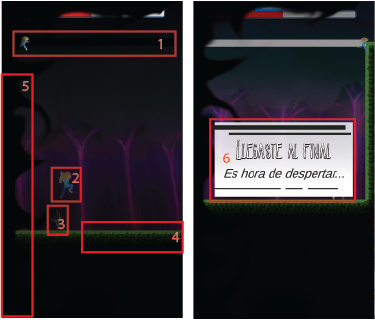
\includegraphics{imgs/hud-pesadilla.png}
    \caption{Interfaz: Pesadilla}
    \label{fig:hud-pesadilla}
\end{figure}

En la Figura~\ref{fig:hud-pesadilla} vemos las pantallas del minijuego asociado a las pesadillas que sufre Lucía. Los elementos en estas pantallas son:\\
1.- \textbf{Barra de Progreso:} Indica cuanto le falta al jugador para llegar al final del minijuego.\\
2.- \textbf{Lucía:} Representa al personaje de Lucía.\\
3.- \textbf{Obstáculo:} Obstáculo que Lucía debe saltar y evitar.\\
4.- \textbf{Terreno:} Terreno por el cuál Lucía va corriendo.\\
5.- \textbf{Oscuridad:} Tentáculos y sombra que viene asechando a Lucía.\\
6.- \textbf{Cuadro de Game Over:} Cuadro que indica que el minijuego ha acabado.

\newpage
\begin{figure}[ht]
    \centering
    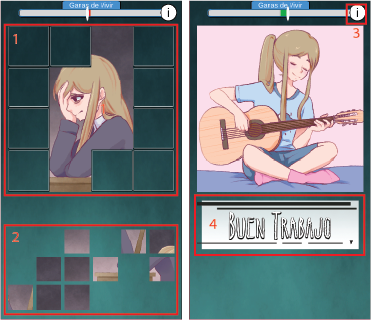
\includegraphics{imgs/hud-puzzle.png}
    \caption{Interfaz: Recuerdos}
    \label{fig:hud-recuerdos}
\end{figure}

En la Figura~\ref{fig:hud-recuerdos} vemos las pantallas del minijuego de los recuerdos de Lucía. Los elementos aquí son:\\
1.- \textbf{Zona de Juego:} Es la zona a la que los jugadores deben arrastrar las piezas para armar el puzzle.\\
2.- \textbf{Piezas:} Zona donde están las piezas del puzzle.\\
3.- \textbf{Pista:} Botón que da una pista al jugador. En este caso muestra una miniatura del puzzle solucionado al mantenerlo presionado.\\
4.- \textbf{Cuadro de Game Over:} Cuadro que indica que el puzzle ha sido completado exitosamente.

\newpage
\begin{figure}[ht]
    \centering
    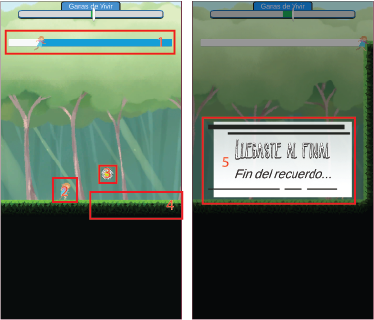
\includegraphics{imgs/hud-pequena.png}
    \caption{Interfaz: Lucía Pequeña}
    \label{fig:hud-pequena}
\end{figure}

La Figura~\ref{fig:hud-pequena} muestra las pantallas del minijuego de Lucía Pequeña, que presenta los siguientes elementos:\\
1.- \textbf{Barra de Progreso:} Indica cuanto le falta al jugador para terminar el minijuego.\\
2.- \textbf{Lucía Pequeña:} Es el personaje que controla el jugador.\\
3.- \textbf{Coleccionable:} Flor que el jugador debe ir recolectando.\\
4.- \textbf{Terreno:} Terreno por el cual Lucía pequeña va corriendo.\\
5.- \textbf{Cuadro de Game Over:} Cuadro que indica el final del minijuego.

\newpage
\begin{figure}
    \centering
    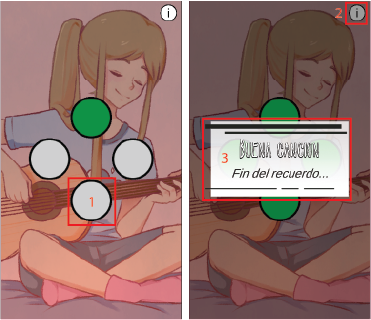
\includegraphics{imgs/hud-musica.png}
    \caption{Interfaz: Música}
    \label{fig:hud-musica}
\end{figure}

La Figura~\ref{fig:hud-musica} muestra las pantallas del minijuego de Música, que presenta los siguientes elementos:\\
1.- \textbf{Botón:} Botón que debe pulsarse siguiendo la secuencia que indica el juego.\\
2.- \textbf{Pista:} Botón que otorga una pista al jugador, en este caso repite la secuencia que se debe seguir.\\
3.- \textbf{Cuadro de Game Over:} Cuadro que indica el final del minijuego.

%%%%%%%%%%%%%%%%%%%%%%%%%%%%%%%%%%%%%%%%%%%%%%%%%%%%
\newpage
\subsection{Game Layout Charts}

\begin{figure}[h!]
    \centering
    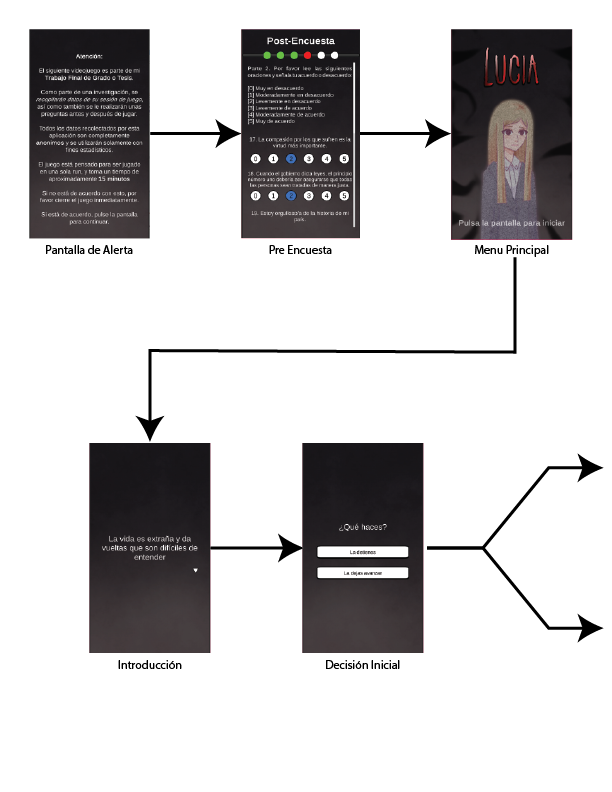
\includegraphics[scale=0.7]{imgs/general-chart-1.png}
    \caption{Flujo General: Inicio}
    \label{fig:chart-1}
\end{figure}

Podemos representar el flujo del videojuego en 3 bloques generales, el inicio del videojuego (Figura~\ref{fig:chart-1}) en el cuál se realiza una alerta inicial al jugador de que el videojuego que está a punto de jugar forma parte de una investigación. Si el jugador continua en la aplicación, se procede a hacer una encuesta previa al inicio del juego, esta encuesta aparece solamente la primera vez que se abre el juego y se rellena una sola vez. Después de la encuesta llegamos al menú principal, desde el cuál podemos iniciar una nueva partida. La partida inicia con un pequeño texto introductorio, antes de enfrentar al jugador con la primera decisión clave: ``¿Salvas a la Chica?''.

\begin{figure}[h!]
    \centering
    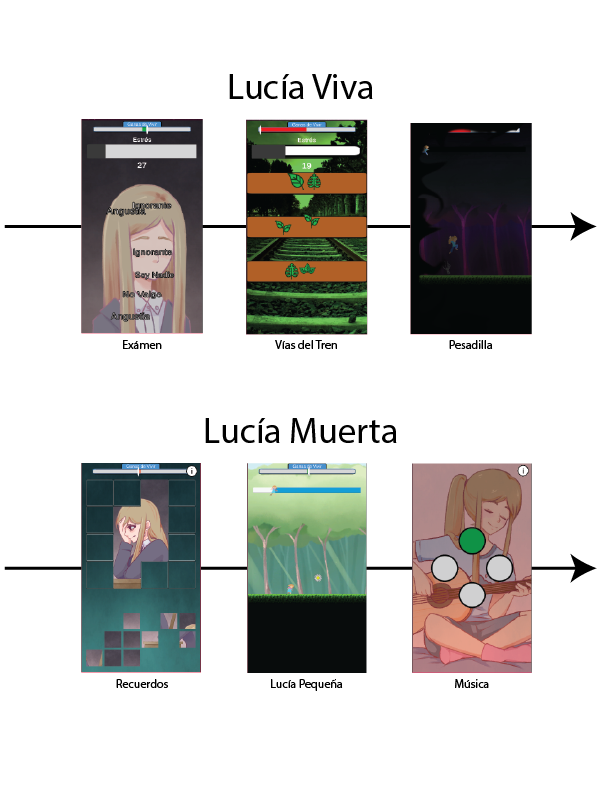
\includegraphics[scale=0.7]{imgs/general-chart-2.png}
    \caption{Flujo General: Minijuegos}
    \label{fig:chart-2}
\end{figure}

Después de esto, pasamos a la segunda sección (Figura~\ref{fig:chart-2}). Aquí tenemos dos rutas posibles dependiendo de la elección que se hizo en la sección anterior, la ruta donde la chica vive, y la ruta donde la chica muere. En ambas rutas se intercalan pantallas de diálogos y narrativa con minijuegos, pero por simplicidad, en el gráfico se muestran solamente los 3 minijuegos que componen cada ruta.

\begin{figure}[h!]
    \centering
    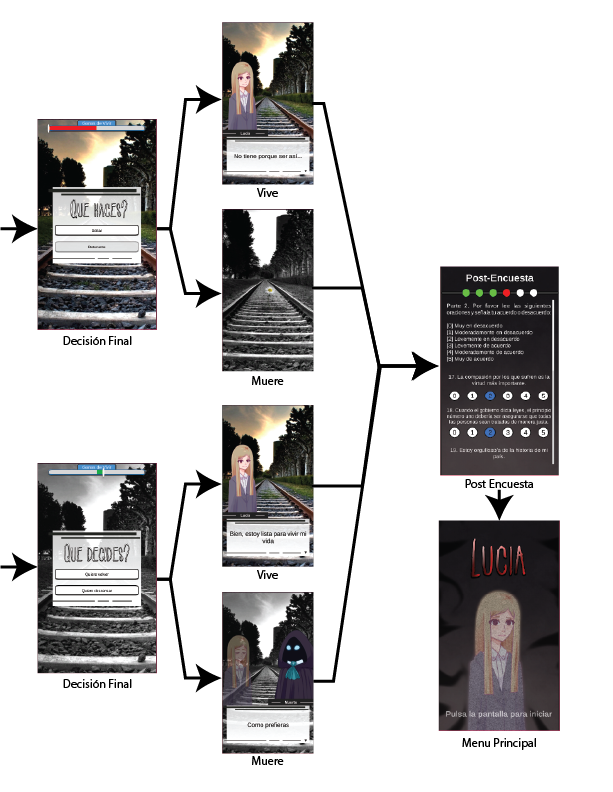
\includegraphics[scale=0.7]{imgs/general-chart-3.png}
    \caption{Flujo General: Final}
    \label{fig:chart-3}
\end{figure}

Al término de cualquiera de las dos rutas se le vuelve a hacer la misma pregunta inicial al jugador, si desea dejar que la chica viva o muera, generando así 4 finales posibles (Vive-Muere, Vive-Vive, Muere-Vive, Muere-Muere). Como se aprecia en la Figura~\ref{fig:chart-3} después de cualquiera de estos finales, se le realiza una encuesta post-juego al jugador (la cuál ocurre solo la primera vez que juega) y se regresa a la pantalla de inicio, dando por terminado el flujo completo del juego. 

%%%%%%%%%%%%%%%%%%%%%%%%%%%%%%%%%%%%%%%%%%%%%%%%%%%%
\newpage
\subsection{Niveles y Ambientes}
El juego cuenta con 4 ambientes principales:

\begin{itemize}
    \item \textbf{Habitación de Lucía:} Aquí transcurren escenas de la historia, así como también el minijuego de la música. Tiene variantes gráficas de día y de noche.
    \item \textbf{Sala de Clases:} Aquí transcurre una escena de la historia, así como también el minijuego del estrés.
    \item \textbf{Vías del Tren:} Aquí transcurre mayor parte de la historia, así como también el minijuego para relajarse después de la prueba, y el minijuego de Lucía Pequeña. Tiene 4 variaciones gráficas dependiendo del tiempo de la historia.
    \item \textbf{Pesadilla:} Aquí transcurre el juego de la pesadilla de Lucía.
\end{itemize}

\begin{figure}[h]
    \centering
    \begin{minipage}{.22\textwidth}
        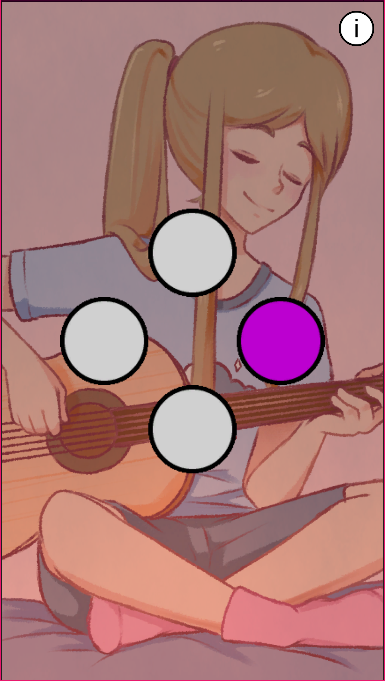
\includegraphics[width=\textwidth]{imgs/screenshot14.png}
    \end{minipage}
    \begin{minipage}{.22\textwidth}
        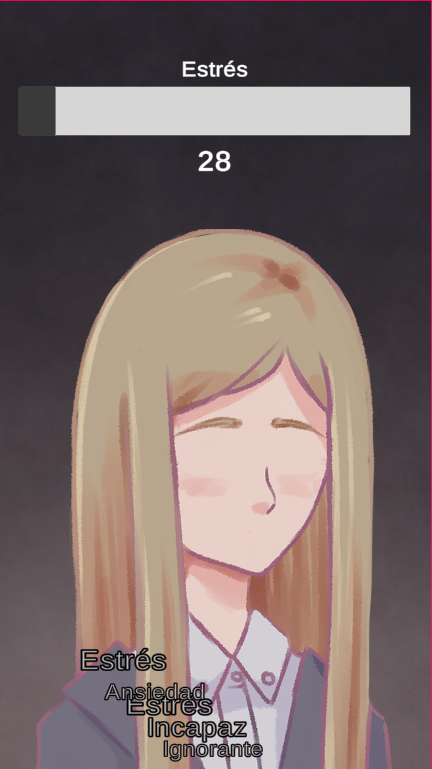
\includegraphics[width=\textwidth]{imgs/screenshot03.png}
    \end{minipage}
    \begin{minipage}{.22\textwidth}
        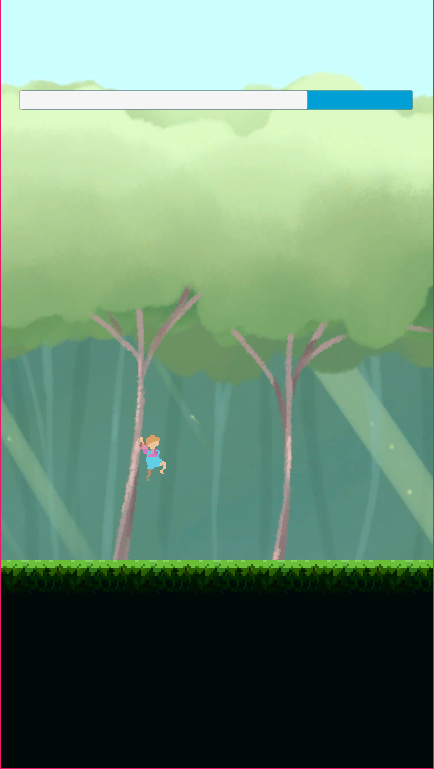
\includegraphics[width=\textwidth]{imgs/screenshot10.png}
    \end{minipage}
    \begin{minipage}{.22\textwidth}
        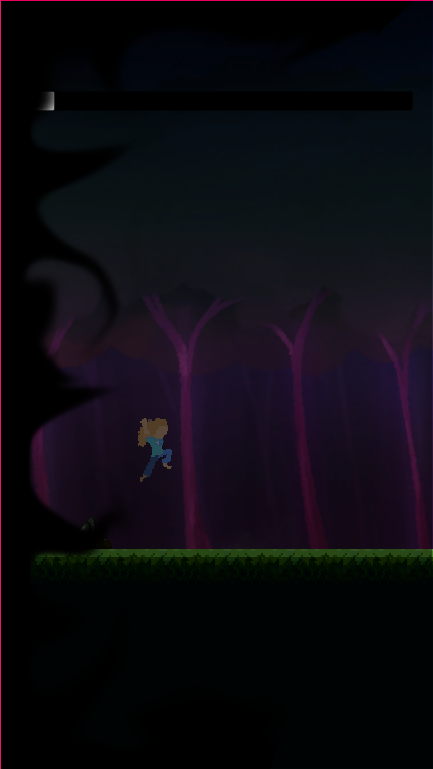
\includegraphics[width=\textwidth]{imgs/screenshot05.png}
    \end{minipage}
    \caption{Ambientes en los minijuegos}
    \label{multifig:ambientes}
\end{figure}

En lo que a niveles respecta, el juego cuenta con 3 minijuegos que contienen una secuencia de niveles:
\begin{itemize}
    \item \textbf{Recuerdos:} En este minijuego el jugador debe resolver un puzzle, se deben resolver 3 puzzles antes de avanzar en la historia, el primero de 3x3, y los dos consecutivos de 4x4 (Figura~\ref{multifig:puzzle-level}).
    \item \textbf{Pesadilla y Lucia Pequeña:} Ambos minijuegos están basados en el mismo nivel, una planicie de 90 unidades de largo en la cuál se instancian obstáculos o coleccionables de manera aleatoria a medida que el jugador avanza (Figura~\ref{fig:run-level}).
\end{itemize}

\begin{figure}
    \centering
    \begin{minipage}{.3\textwidth}
        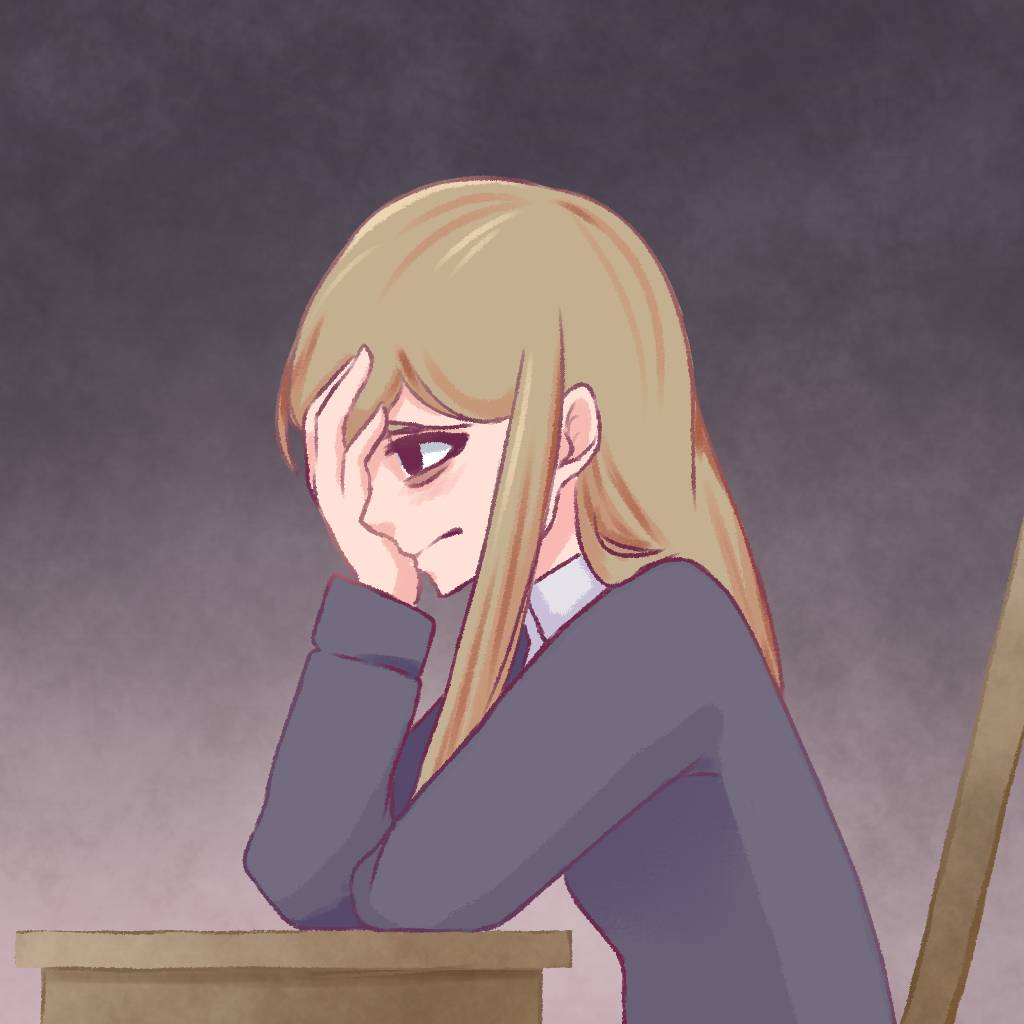
\includegraphics[width=\textwidth]{imgs/Memory1.png}
    \end{minipage}
    \begin{minipage}{.3\textwidth}
        \includegraphics[width=\textwidth]{imgs/Memory2.png}
    \end{minipage}
    \begin{minipage}{.3\textwidth}
        \includegraphics[width=\textwidth]{imgs/Memory3.png}
    \end{minipage}
    \caption{Niveles de Puzzle}
    \label{multifig:puzzle-level}
\end{figure}

\begin{figure}
    \centering
    \includegraphics[width=\textwidth]{imgs/run-level.png}
    \caption{Nivel de correr}
    \label{fig:run-level}
\end{figure}


%%%%%%%%%%%%%%%%%%%%%%%%%%%%%%%%%%%%%%%%%%%%%%%%%%%%
\subsection{Objetos}
El juego se desarrolla principalmente en las pantallas de narrativa, las cuales se vieron en detalle en la Sección~\ref{sec:pantallas}. En el caso de los minijuegos podemos encontrar los siguientes objetos:

\begin{itemize}
    \item \textbf{Hoja:} Aparece en el minijuego de las vías del tren, cuando Lucía está viva. Este objeto simula las hojas de los árboles con las que Lucía juega (Figura~\ref{fig:hoja}).
    \item \textbf{Mano:} Aparece en el minijuego de la pesadilla, cuando Lucía está viva. Son los obstáculos que el personaje debe saltar y buscaban tener un estilo tenebroso/de miedo (Figura~\ref{fig:mano}).
    \item \textbf{Flor:} Aparece en el minijuego de Lucía Pequeña, cuando Lucía está muerta. Son los objetos que el personaje debe recolectar, simboliza las flores que habían en el lugar donde Lucía jugaba de pequeña (Figura~\ref{fig:flor}).
\end{itemize}

\begin{figure}[h]
    \centering
    \begin{minipage}{.25\textwidth}
        \includegraphics[width=\textwidth]{imgs/hoja.png}
        \caption{Hoja}
        \label{fig:hoja}
    \end{minipage}
    \begin{minipage}{.25\textwidth}
        \includegraphics[width=\textwidth]{imgs/hand.png}
        \caption{Mano}
        \label{fig:mano}
    \end{minipage}
    \begin{minipage}{.25\textwidth}
        \includegraphics[width=\textwidth]{imgs/daisy.png}
        \caption{Flor}
        \label{fig:flor}
    \end{minipage}
\end{figure}

%%%%%%%%%%%%%%%%%%%%%%%%%%%%%%%%%%%%%%%%%%%%%%%%%%%%
\subsection{Producción Externa}
La mayoría de los elementos que han sido mencionados en este documento han sido desarrollados por el equipo de trabajo. No obstante, una serie de ellos es necesario que sean producidos por terceros, estos elementos son:

\begin{itemize}
    \item \textbf{Música y Efectos Sonoros:} En particular, es necesario que se desarrollen los siguientes elementos:
    \begin{itemize}
        \item Tema Principal (utilizado en el menú principal)
        \item Música de ambiente para la narrativa.
        \item Música para el minijuego de estrés.
        \item Música para el minijuego de las vías del tren.
        \item Música para el minijuego de la pesadilla.
        \item Música para el minijuego de los recuerdos de Lucía.
        \item Música para el minijuego de Lucía Pequeña.
        \item Música de ambiente para el minijuego de la Música.
        \item Efecto de Sonido cuando Lucía salta (Pesadilla + Lucía Pequeña)
        \item Efecto de Sonido cuando Lucía choca con un obstáculo (Pesadilla)
        \item Efecto de Sonido cuando Lucía pequeña recolecta un coleccionable.
        \item Efecto de Sonido al completar un puzzle.
        \item Efecto de Sonido al superar un minijuego.
    \end{itemize}
    \item \textbf{Efectos de Partículas:} Partículas que dan una mejor sensación de feedback al jugador, vuelven al juego más pulido y aportan en la estética, en particular son necesarias las siguientes:
    \begin{itemize}
        \item Partículas de ``Oscuridad''
        \item Efecto cuando el jugador presiona la pantalla.
        \item Efecto de ``Viento'' cuando el jugador se encuentra al aire libre (Vías del tren).
    \end{itemize}
\end{itemize}

%%%%%%%%%%%%%%%%%%%%%%%%%%%%%%%%%%%%%%%%%%%%%%%%%%%%

\newpage
\subsection{Encuestas}

Nuestro segundo objetivo era diseñar y realizar un estudio con cuestionarios pre- y post- juego que nos permitiera analizar el comportamiento del jugador. Para ellos hemos integrado una encuesta en el videojuego como se apreció en la Sección~\ref{sec:pantallas}.  Las encuestas aparecen automáticamente la primera vez que el jugador juega al videojuego, y la primera vez que lo completa.

Se ha decidido integrar las encuestas dentro del videojuego ya que es una forma más cómoda para la recolección de los datos de parte del usuario en lugar de utilizar una plataforma externa como Google Forms o Survey Monkey, debido a que mantenemos al usuario completamente inmerso dentro de la aplicación. Además eliminamos factores externos (dentro del mismo móvil) que pudiesen distraer al usuario al estar cambiado entre aplicaciones, tal como lo sería revisar sus redes sociales, responder mensajes, ver notificaciones, que al usuario se le olvide responder las encuestas, e incluso que pueda responder las encuestas en el orden equivocado.

\begin{figure}[h]
    \centering
    \includegraphics[width=\textwidth]{imgs/encuesta.png}
    \caption{Pantallas Encuesta \acrshort{mfq}}
    \label{fig:pantallas-encuesta}
\end{figure}

Como la encuesta se respondería desde el móvil, la prioridad al momento de investigarla y diseñarla fue que fuese basada en una escala, ya que este método de respuesta es más práctico para ejecutar desde el móvil en contraste a escribir una respuesta abierta o una opinión (la cuál es más cómoda en dispositivos como un computador, o una tablet).

De acuerdo a las recomendaciones hechas por el articulo ``Measuring morality in videogames research''\cite{measure-morality} se escogió el \gls{moral-foundation}\cite{moral-foundation} como test para esta investigación. Este test consta de 32 preguntas basadas en una escala utilizado múltiples veces en distintas investigaciones relacionadas con videojuegos (Kremar y Cingel\cite{kremar-cingel}, Joeckel et al.\cite{joeckel}, Weaver y Lewis\cite{weaver-lewis}, Grizzard et al.\cite{grizzard}) que nos ofrece una manera robusta de testear la moralidad así como también ser accesible y cómoda para su implementación dentro del juego.

En la Figura~\ref{fig:pantallas-encuesta} se observan las pantallas de la encuesta, y como posee una barra de progreso que permite al usuario tener una noción de cuanto lleva y cuanto le falta por responder.
